%!TEX root = ../TTK4900-MHT.tex

\chapter{MHT Module}\label{chapter:mht-module}
To create a complete tracking \emph{system}, rather than a tracking \emph{\gls{algorithm}}, it is often necessary to complement the main algorithm with support modules. The system, or module if it is a part of a bigger system, presented here is an extension of the pre master project~\cite{Liland_2017}. The aim of this chapter is to provide a complete walkthrough of the the track oriented MHT system developed in this thesis. This \gls{mht} module is based on both radar and \gls{ais} data from sensors mounted on own vessel. Since the radar is one of the most trustworthy sensors on board any vessel is this tracking module based on radar measurement primarily, with the \gls{ais} as an aiding system. This approach guided some of the design choices made throughout the development of the module. 

The motion model which is used throughout the entire tracking system when predicting and filtering target behaviour is presented first. Next follows an overview of the algorithm used to initiate new tracks into the MHT algorithm, followed by the entire MHT tracking algorithm with all its sub-routines.

It will be assumed throughout this thesis that radar data is processed, as outlined in Section~\ref{sec:radar_preprocessing}, into a set of points. These points is referred to as radar measurements.

\section{Motion Model}\label{sec:motion-model}
\subsection{Reference frame}
A local Cartesian NED-frame, like \gls{utm} will be used throughout this thesis, with the assumption than all input sensors are transformed to this frame (see Section~\ref{subsec:frame_conversion}). This local projection from a geodetic coordinate system to a Cartesian coordinate system is acceptable as long as the area the system is working on is within one grid. A global geodetic frame, like WGS84 would be preferable in situations where the system tracks object over world-scale lengths but would yield non-linear equations of motion.

\subsection{Constant velocity model}
A target's state (\ref{eq:state_vector}) is modelled with position and velocity in a 2D Cartesian frame where the positive \(x\)-axis is pointing east and the positive \(y\)-axis is pointing north. The two latest states are the velocities in their respective direction.
\begin{equation}
\V{x} = \begin{bmatrix}
x & y & \dot{x} & \dot{y}
\end{bmatrix}^T
\label{eq:state_vector}
\end{equation}

Since modelling the behaviour of any ship under unknown command is next to impossible, a common assumption in tracking theory is that every target will continue on as usual, more precisely that their velocity is constant. Although simple, this model captures the essence of most vessels at sea, and it should be noted that both maritime training~\cite{Allen2005} and regulation~\cite{IMO1972} dictates that vessels should hold steady course and change course in clear decisive turns. This model is also very common in tracking applications and is used in~\cite{Reid1979,Coraluppi2000,Brekke2012,Wilthil,Vo2015,Chen2003,Habtemariam2015} among others. To give room in our model for manoeuvring, process noise is introduced with covariance set according to the assumed manoeuvring capabilities of the vessels. This could be set as a fixed value for all targets, as done in this work, or estimated based on the history of the track or AIS information. This behaviour can be modelled as a linear time invariant system with time evolution (\ref{eq:motion_model}), measurement model (\ref{eq:measurement_model}), transition and observation matrices (\ref{eq:model_matrices}), and system and measurement noise matrices (\ref{eq:noise_matrices}).

\begin{equation}\label{eq:motion_model}
\V{x}_{k+1} = \M{\Phi} \V{x}_k + \V{w}_k \qquad \V{w} \sim \mathcal{N}(0;\M{Q})
\end{equation}
\begin{equation}\label{eq:measurement_model}
\V{z}_{k+1} = \M{H}\V{x}_k + \V{v}_k \qquad \V{v} \sim \mathcal{N}(0;\M{R})
\end{equation}
\begin{equation}\label{eq:model_matrices}
\M{\Phi} =	\begin{bmatrix}
1 & 0 & T & 0 \\
0 & 1 & 0 & T \\
0 & 0 & 1 & 0 \\
0 & 0 & 0 & 1 \\
\end{bmatrix}
\quad
\M{H} =	\begin{bmatrix}
1 & 0 & 0 & 0 \\
0 & 1 & 0 & 0 \\
\end{bmatrix}
\end{equation}
\begin{equation}\label{eq:noise_matrices}
\M{Q}	= \sigma_v^2 \begin{bmatrix}
\frac{T^3}{3} 	& 0 				& \frac{T^2}{2}	& 0 			\\
0 				& \frac{T^3}{3}  	& 0 			& \frac{T^2}{2}	\\
\frac{T^2}{2}	& 0					& T				& 0				\\
0				& \frac{T^2}{2}		& 0				& T				\\
\end{bmatrix}
\quad
\M{R} =	\sigma_m^2 
\begin{bmatrix}
1 & 0 \\
0 & 1 \\
\end{bmatrix}
\end{equation}
\begin{equation*}
\begin{split}
\M{\Phi} 	&= \text{state transition matrix} \\
\M{H}		&= \text{state observation matrix} \\
\M{Q}		&= \text{system covariance matrix} \\
\V{w}		&= \text{\gls{system noise}} \\
\V{v}		&= \text{\gls{measurement noise}} \\
\V{z}		&= \text{measurement vector} \\
k 			&= \text{time index} \\
T  			&= \text{time step} \\
\end{split}
\end{equation*}

\section{Track Initiation}
In comparison with \gls{homht}, which treats every measurement as a potential new track. \Gls{tomht} does not have any built-in initialization of tracks since it only maintains already existing tracks with track splitting and measurement-to-track association for every scan. To remedy this lack, we need an algorithm that can find consistent and predictable patterns in an assumed uniformly distributed measurement space of clutter. 

In this work, new tracks are initiated with 2/2 \& m/n logic~\cite{Vo2015} on the unused measurements after each MHT iteration. As the name of the method indicates, this is a two step verification, where the first act as a rough filter and the second as a fine filter. As a common in most tracking systems, the radar clutter is assumed uniformly distributed in the measurement area. 
%This assumption is quite rough in the radial measurement space, and even worse approximation in Cartesian measurement space, as illustrated in \Cref{fig:clutter_radial,fig:clutter_cartesian}.  Although far from perfect, tests shows that we still get satisfactory performance from the 2/2\&m/n method.
% \begin{figure}[H]
% \centering
% \begin{minipage}{0.45\textwidth}
% 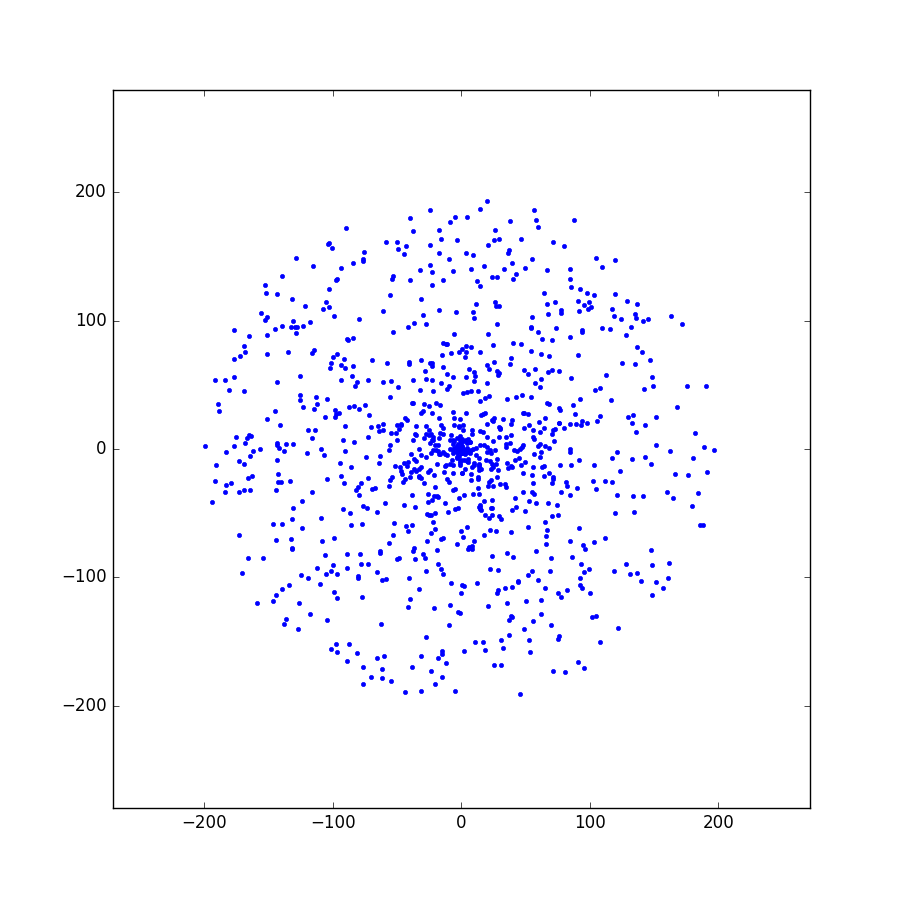
\includegraphics[width=\textwidth]{Figures/clutterRadial.png}
% \caption{Uniform radial clutter}\label{fig:clutter_radial}
% \end{minipage}\hfill
% \begin{minipage}{0.45\textwidth}
% 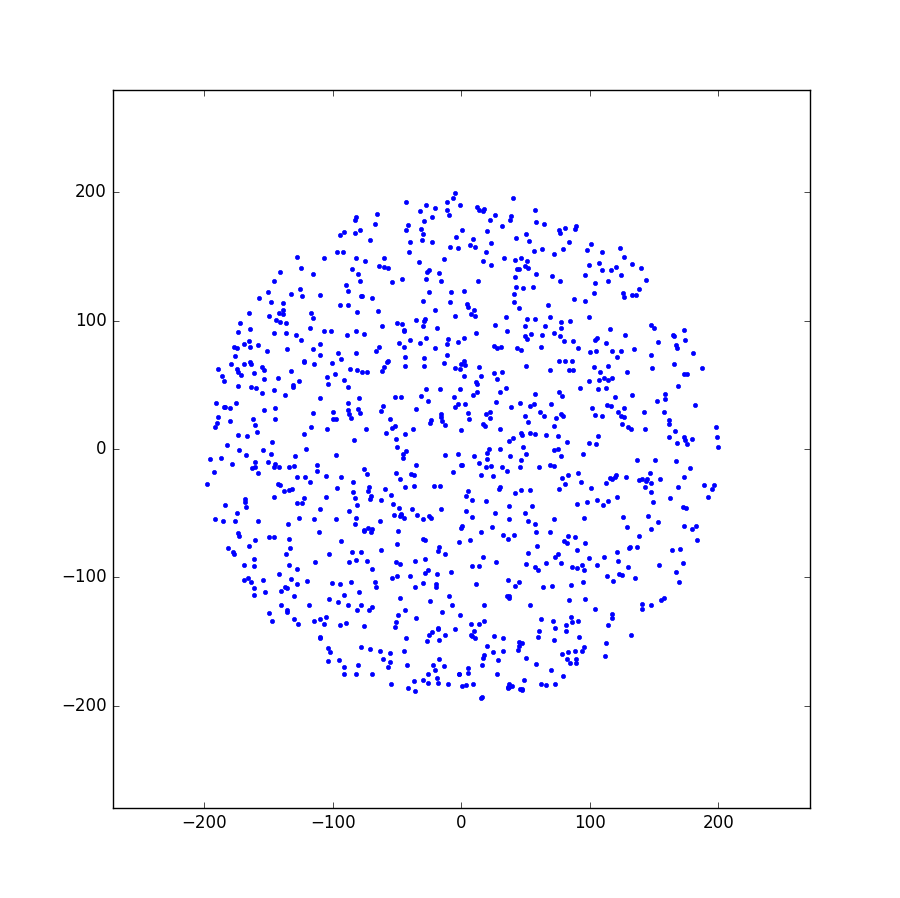
\includegraphics[width=\textwidth]{Figures/clutterCartesian.png}
% \caption{Uniform Cartesian clutter}\label{fig:clutter_cartesian}
% \end{minipage}
% \end{figure}

The flow of the method is illustrated in Figure~\ref{fig:init_flowchart}, and for better clarity, the algorithm is explained from the last step to the first step, since this is the sequence a newly started initiation algorithm will perform its operations.
\begin{figure}[H]
\centering
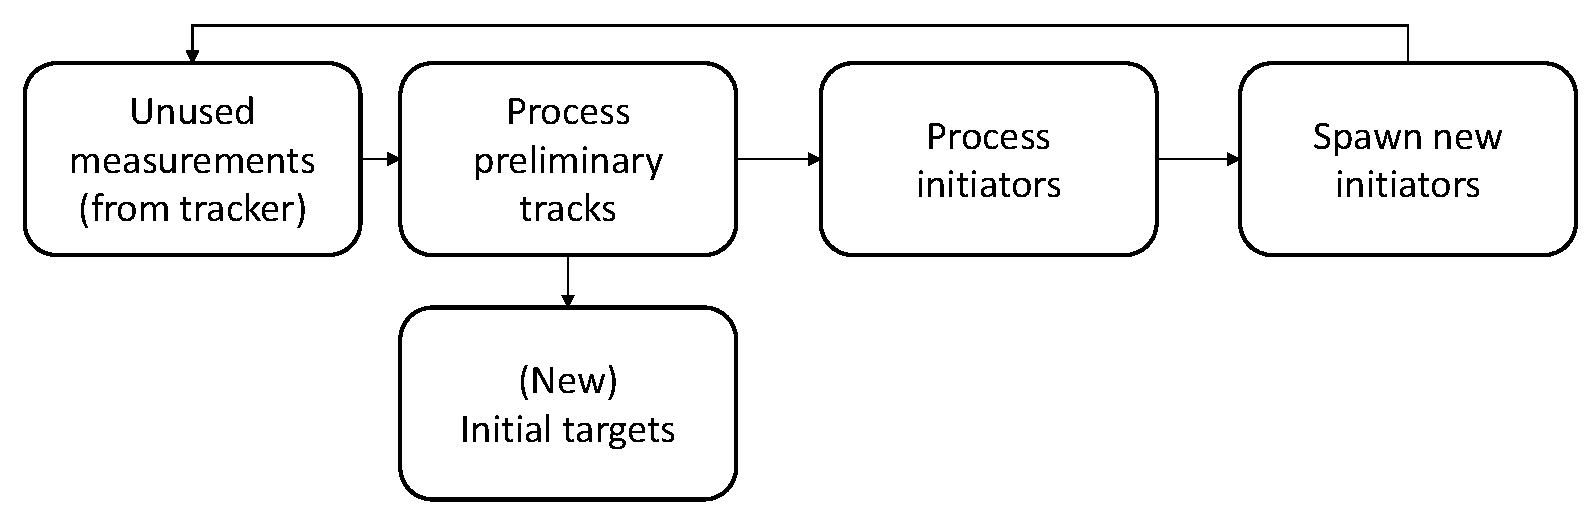
\includegraphics[width = .9\textwidth]{init_flowchart.pdf}
\caption{2/2\&m/n flowchart}\label{fig:init_flowchart}
\end{figure}

\subsection{Spawn new initiators}
All measurement unused by the `Process preliminary tracks' and `Process initiators' steps will be the basis for new \emph{initiators}. An initiator is a measurement that awaits its match in the next scan. The idea is that uniformly distributed clutter will not (often) reappear at approximately the same location two times in a row, effectively filtering out most of the clutter.

\subsection{Process initiators}
When the next scan arrives, all the unused measurements from the `Process preliminary tracks' step will be used as candidates in this step. Since an initiator is only a position and not a full state with velocity, all directions are equally likely, and the only design parameter in this step is maximum speed of targets to be tracked. This parameter sets an outer limit on the circle acting as a gate for the second and confirming measurement. When matching initiators with a second measurement, we want to select the closest measurement, making the assumption that the two consecutive measurements are the most likely to belong together. In a single target scenario, where this would be to calculate the distance to all the alternative measurements and select the lowest, the association is already done. While in a multitarget scenario, we \emph{could} select the closest measurement to any initiator, but we would have to do this one initiator at a time. This would lead to different results depending on the arrangement of the initiators in the programming of this method. A different approach would be to calculate all the different distances for any possible combination of initiators and measurements, sort the list, and assign the distances from the shortest to the longest possible distances. This approach would not be influenced by randomness like the arrangement of the initiators in a programming language, but would not necessarily give the global optimal association regarding the how many initiators that are assigned measurements and their respective distances.

Since we can have situations like exemplified in Figure~\ref{fig:init_gating}, where two initiators have the same measurement inside their gates, and one of them have a second measurement inside its gate, we need to take the global consequence of any assignment into consideration.
\begin{figure}
\centering
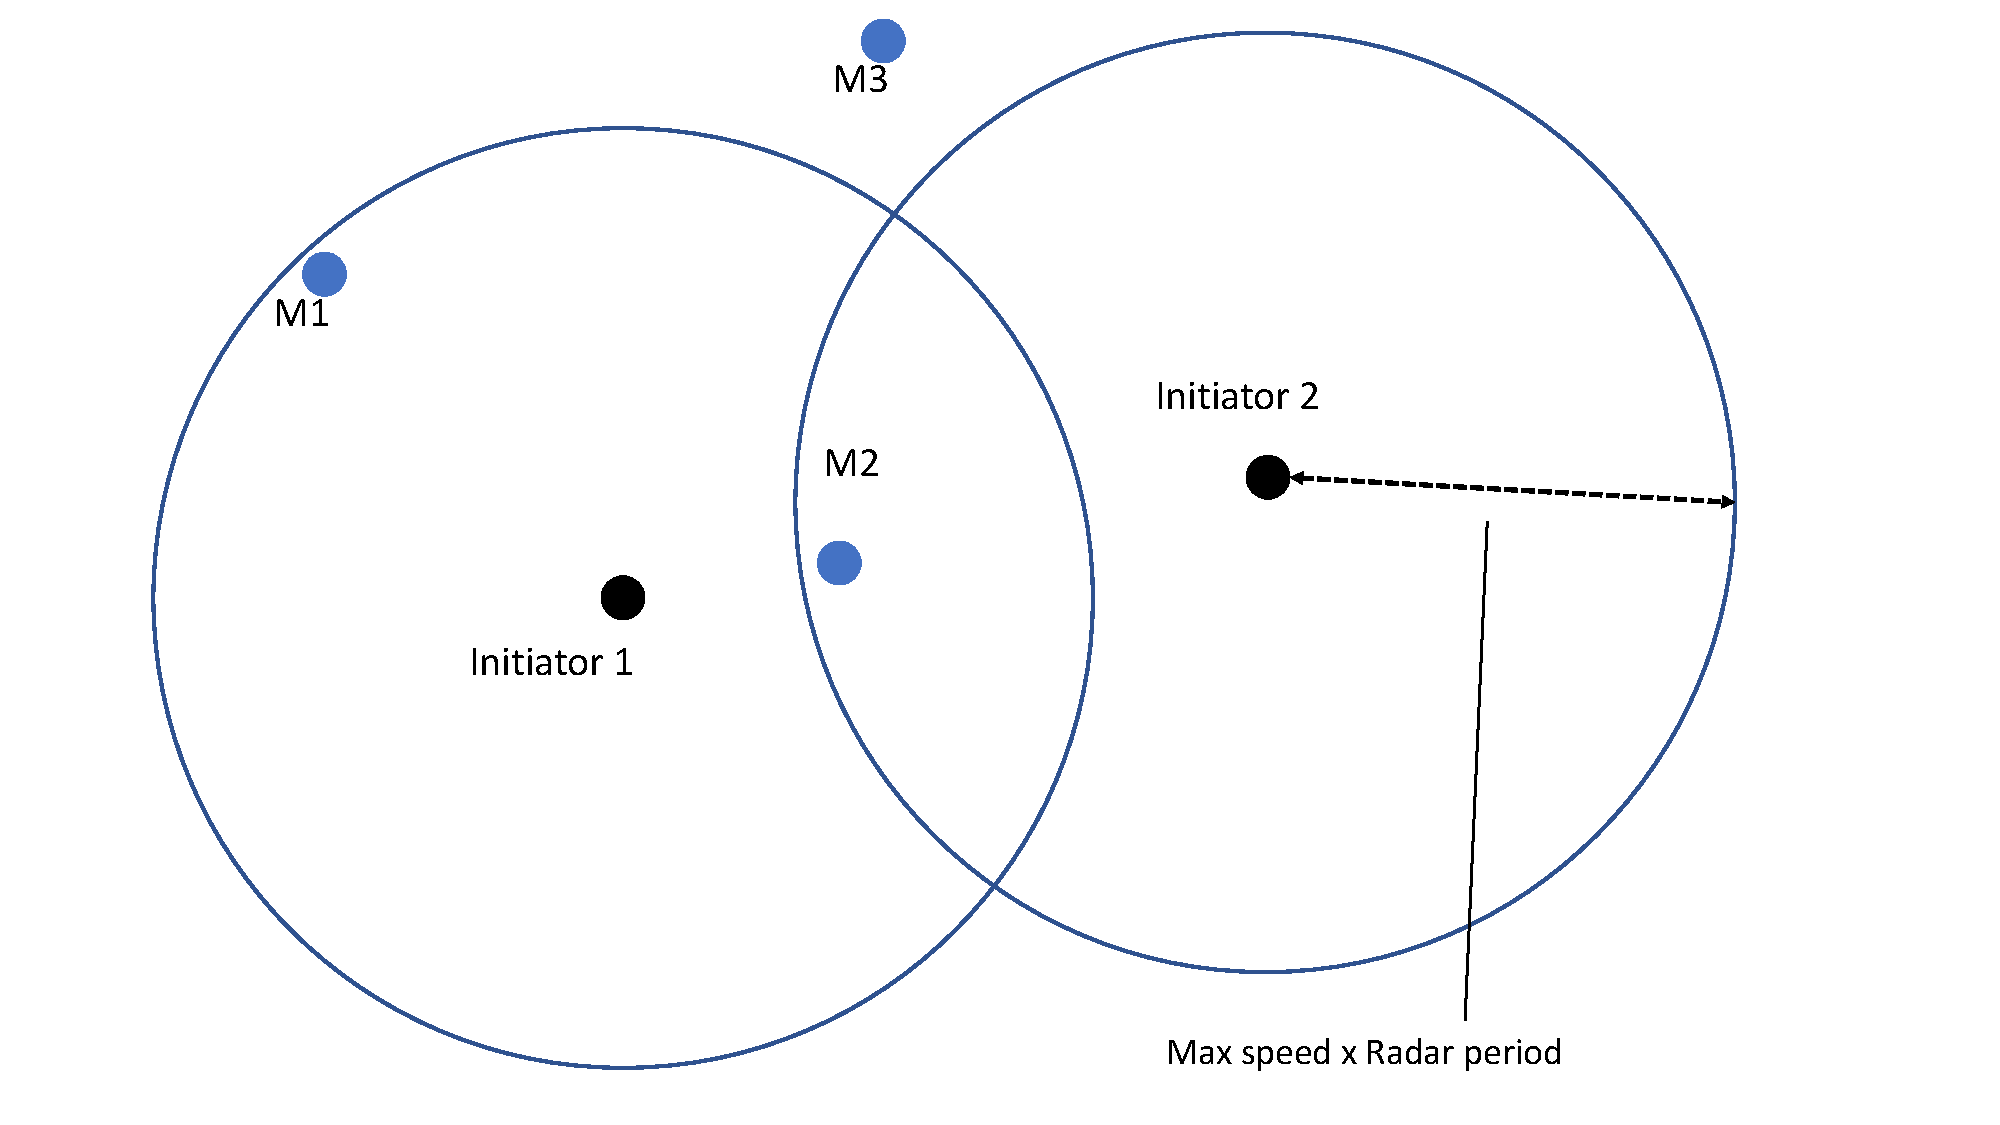
\includegraphics[width = .8\textwidth]{Figures/init_gating.pdf}
\caption{Initiator gating example}\label{fig:init_gating}
\end{figure}
If using method 1; to sequentially select the best, we have two possible outcomes. When starting with initiator 1, this initiator would be associated with measurement 2, and initiator 2 would not be associated with any measurements. On the other hand, starting with initiator 2 would lead to this initiator being associated with measurement 2, and initiator 1 would be associated with measurement 1. This randomness in outcome based on which initiator the algorithm starts with is clearly not a desired property. If using using method 2; to sequentially select the globally shortest distance, we would first associate initiator 1 with measurement 2, and there would not be any measurements left for initiator 2, leaving this empty.

A third option is to formulate the problem as a global combinatorial problem, and use an `off-the-shelf' solution to solve the problem. We have essentially a matrix with initiators along one axis and measurements along the second axis and the distance between them in their intersections, as in (\ref{eq:init_assignment_matrix}) for our example.
\begin{equation}\label{eq:init_assignment_matrix}
\kbordermatrix{
	 	& M_1 	& M_2 	& M_3	\\
    I_1 & 3 	& 1 	& 5 	\\
    I_2 & 7 	& 2 	& 6		\\
}
\end{equation}
The values above the threshold set by the maximum speed multiplied with the time period between the radar scans can be set to infinity to symbolise that this combination is not possible, see (\ref{eq:gated_init_assignment_matrix}) where the gate threshold is 4.
\begin{equation}\label{eq:gated_init_assignment_matrix}
\kbordermatrix{
	 	& M_1 		& M_2 	& M_3		\\
    I_1 & 3 		& 1 	& \infty 	\\
    I_2 & \infty 	& 2 	& \infty	\\
}
\end{equation}
If we remove the columns with only infinity, we are removing measurements that cannot be associated under any circumstances, thus reducing the size of the problem, see (\ref{eq:masked_gated_init_assignment_matrix}). With this pre processing, we want to assign each row to a column so that the sum of the selected intersections are minimal. 
\begin{equation}\label{eq:masked_gated_init_assignment_matrix}
\kbordermatrix{
	 	& M_1 		& M_2	\\
    I_1 & 3 		& 1  	\\ 
    I_2 & \infty 	& 2 	\\
}
\end{equation}
We now have formulated our problem in a way that it can be solved by the `Hungarian'\footnote{also known as the Munkres or Kuhn-Munkres algorithm} algorithm~\cite{Munkres1957}, which will give us the association \(I_1 \rightarrow M_1\) and \(I_2 \rightarrow M_2\). From the associations, a full state and new preliminary track is created with the latest measurement as position and velocity calculated based on the position difference divided by the time difference between the measurements. A preliminary track contains a state, initial covariance and counters of number of checks and passed checks. The initial covariance is a design variable and would be set according to the measurement and process noise.

\subsection{Process preliminary tracks}
When a new set of unused measurements arrive from the tracker, all the preliminary tracks are predicted to the time of the measurements. We now have the same association challenge between the predicted states and the measurements as with the initiators and measurements. Since we now have a full state and covariance for every preliminary track, we calculate the \gls{nis} for every combination of preliminary tracks and measurements, and selects the best combination. The preliminary tracks that are associated with a new measurement, their passed counter is incremented with one, while all preliminary tracks' checks counter is incremented with one. 

For preliminary tracks that have enough passed measurements, a new initial target is sent to the tracker. All preliminary tracks with check counter above the threshold is categorized as dead and deleted. 

\subsection{AIS aiding}
Since we might have AIS data available, it would be desirable to use this to improve the time and reliability of the initialization. In the same way as unused radar measurements are the input to the initialization procedure, we can use the unused AIS measurements to skip the first 2/2 filtering and create a preliminary track for each AIS measurement. This way we are giving the AIS measurements a little more `weight', but as this tracking system is based on AIS \emph{aiding} we still want the m/n filtering to be done with radar measurements. To avoid creating duplicate preliminary tracks for the same \gls{mmsi} over time, only unused AIS measurements with a MMSI not in the preliminary tracks are created. These choices are highly design specific and many other approaches is possible. 


\section{MHT Overview}
\begin{figure}
 \centering
 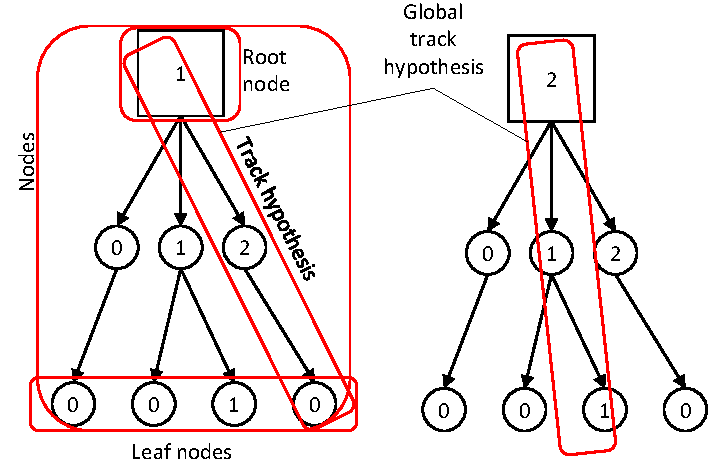
\includegraphics{Figures/Track-tree.pdf}
 \caption{Hypothesis tree}\label{fig:hyp_tree}
\end{figure}
The aim of this section is to outline the major steps in the MHT module and the flow of data and decisions. Figure~\ref{fig:algorithm_flow} shows the main steps that the module perform at each iteration / radar scan. The \gls{mht} algorithm is working on a set of \glspl{dag} or tree structures, often called a forest. The forest contains as many trees as targets the algorithm is tracking. Each tree consist of a root node and a set of child nodes, where each row represent a scan or discrete time. The leaf nodes are referred to as track hypotheses since leaf nodes represents itself and its parents.

 When new AIS and radar measurements are received, all leaf nodes are predicted forward to the time of the radar measurements. The radar measurements are then gated for each leaf node, and new pure radar hypotheses are generated for radar measurements within the gate. Each leaf node are then predicted to the time of the AIS measurements, and are gated at their time. AIS measurements inside the gate are then predicted to the time of the radar measurements where the radar measurements are gated based on each of the filtered AIS measurements. For each gated radar measurements give rise to fused hypotheses and from each AIS measurements without any radar measurement inside its gate a pure AIS hypothesis is created. Each new hypothesis is then given a score, which is the cumulative score of the parent node score and the new node's score. The target trees are then clustered according to which trees that shares measurements, whereon clusters with only one tree has the option of removing / merging similar hypotheses to reduce the size of the tree. For each cluster, the cluster-wise globally best association combination is selected using \gls{ilp}. Then, for each selected hypothesis the parent N steps above becomes the new root of that tree, and the unused children to the previous root node are removed. Next, targets whose best hypothesis have a score below the threshold is terminated, followed by the initialization of new targets from the initiator module. 

 The algorithm described in the three following sections are repeated for every leaf node in the forest. To avoid an extensive use of node- and measurement indexing the procedure is explained for one leaf node, with this node referred to as c---node, and is repeated for all leaf nodes in the forest. The c is only a symbol for indexing and referencing the chosen leaf node relative to predicted and filtered states. 
\begin{figure}[H]
\centering
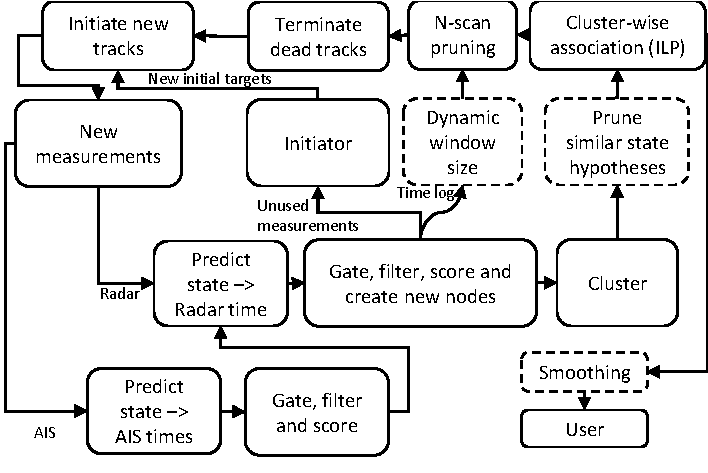
\includegraphics[width = \textwidth]{algorithm_flowchart.pdf}
\caption{Algorithm flowchart}\label{fig:algorithm_flow}
\end{figure}

To illustrate how this \gls{mht} system works we can look at an example of a target when it is turning. Figure~\ref{fig:hypotheses_when_turning} shows a single target which started in the lower left side doing a hard port turn followed by a straight course. The purple dots is the true track, the black dot is the stating position, the solid line is the selected/best hypothesis and the dotted lines are all the other hypotheses. As the target is turning, the zero hypotheses will continue in a straight line to allow for the possibility that there is a missed detection at that time. Most of the zero hypotheses are also splitting after their first and second scan upon creation, which can be seen as sharp angles between dotted lines moving outwards in the turn and dotted lines representing hypotheses which have re-connected with the true target.
\begin{figure}[H]
\centering
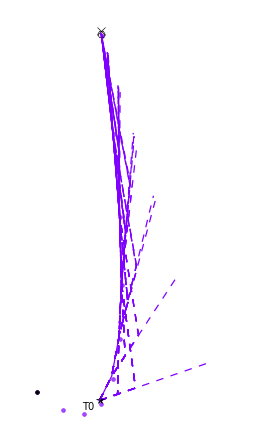
\includegraphics[height = .5\textheight]{Figures/Hypotheses_when_turning.PNG}
\caption{Hypotheses when turning}\label{fig:hypotheses_when_turning}
\end{figure}

\section{Process radar measurements}\label{sec:process_radar_measurements}
\subsection{Predict to radar time}
To compare new radar measurements with existing hypotheses, we should predict their states to the same time as the radar measurements, which can be done with the Kalman filter `time update' equation (\ref{eq:kalman_timeUpdate}) and the motion model from Section~\ref{sec:motion-model}. The residual covariance (\ref{eq:residual_covariance}), which is a part of the `measurement update' sequence of a Kalman filter are also calculated as the residual covariance is needed in the gating and these matrices are not dependent on the measurement residual.
\begin{equation}\label{eq:kalman_timeUpdate}
\begin{split}
\V{\bar{x}}_1 	&= \M{\Phi}(\Delta T_R) \V{x}_c \\
\M{\bar{P}}_1	&= \M{\Phi}(\Delta T_R) \M{P}_c \M{\Phi}^T(\Delta T_R) + \M{Q}(\Delta T_R) \\
\end{split}
\end{equation}
\begin{equation}\label{eq:residual_covariance}
\M{S}_1	= \M{H}\M{\bar{P}}_1 \M{H}^T + \M{R}_{Radar}
\end{equation}
\begin{equation*}
\begin{split}
\V{\bar{x}}		&= \text{predicted state} \\
\V{x}_c 		&= \text{origin node state} \\
\M{\bar{P}} 	&= \text{predicted state covariance} \\
\M{P}_c 		&= \text{origin node state covariance} \\
\Delta T_R 		&= \text{Radar time period} \\
\end{split}
\end{equation*}

\subsection{Gate}
To limit the number of hypotheses the leaf node have to create, the measurements are gated based on the leaf node's predicted covariance and a set confidence value. The size of the gate (Figure~\ref{fig:gating_radar_at_radar_time}) will reflect how insecure the prediction is, which is a function of how many detections and missed detections the leaf node and its parents have had. The gate (\ref{eq:gate}) is defined as \gls{nis} less than a threshold set by the inverse \(\chi^2\)--distribution \gls{cdf} with as many degrees of freedom as the measurement, two degrees of freedom for a maritime radar, and a set confidence value. A set of confidence levels and belonging \(\chi^2\) \gls{cdf} values are listed in Table~\ref{tab:chi_square}. The measurement residual and \gls{nis} is calculated for each measurement, and the measurements that does not pass the test are discarded.
\begin{figure}
\centering
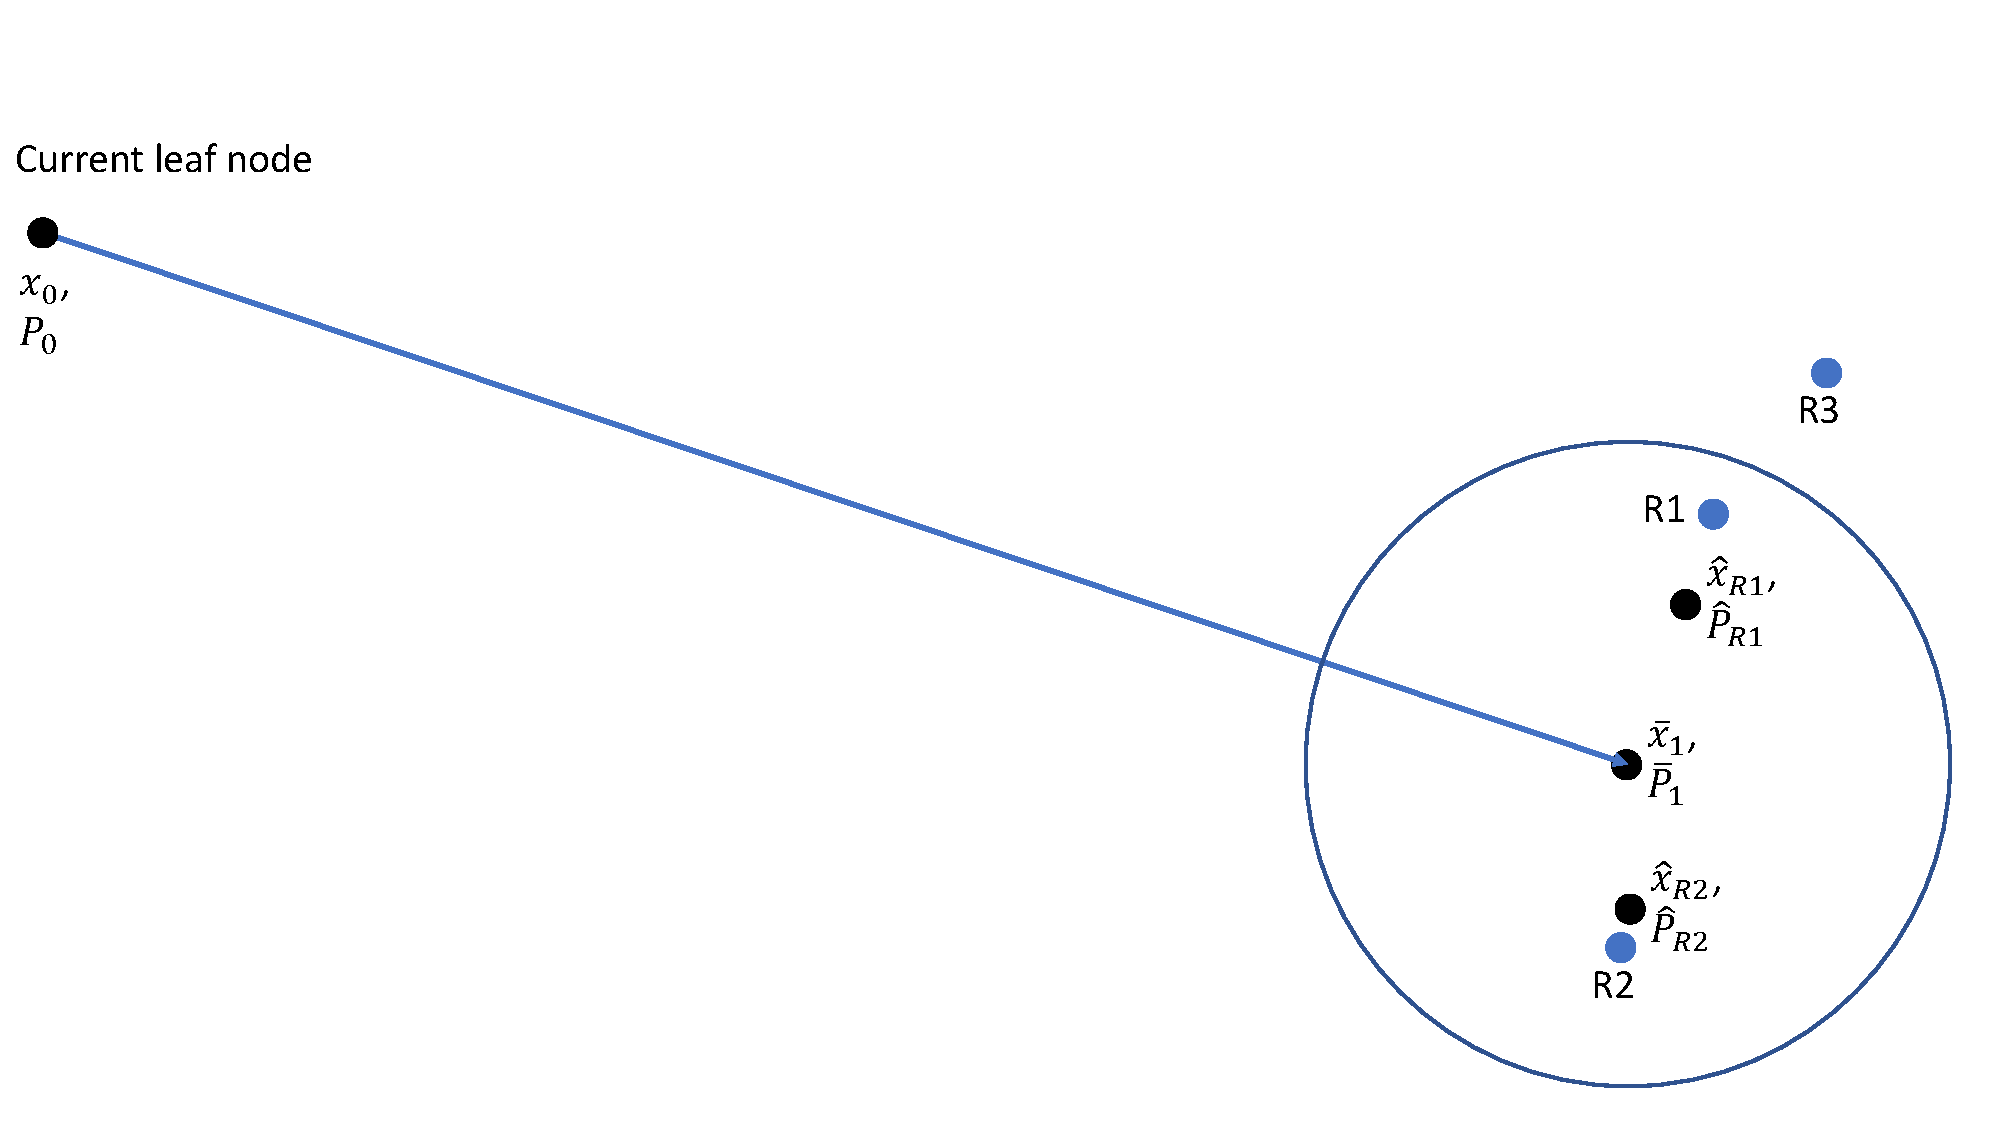
\includegraphics[width = .8\textwidth]{Figures/radar_gating.pdf}
\caption{Gating radar measurements at radar time}\label{fig:gating_radar_at_radar_time}
\end{figure}
\begin{equation}\label{eq:gate}
\begin{gathered}
\V{\tilde{z}} = \V{z} - \M{H}\V{\bar{x}}_1 \\
NIS = \V{\tilde{z}}^T	\M{S}^{-1} \V{\tilde{z}} \leq \eta^2
\end{gathered}
\end{equation}
\begin{equation*}
\begin{split}
\V{\tilde{z}}	&= \text{Measurement residual} \\
\eta^2 			&= \text{Gate size} \\
\end{split}
\end{equation*}
\begin{table}
\centering
\begin{tabular}{c c c c c c c c}
Confidence 	& 70\% 	& 80\% 	& 90\% 	& 95\% 	& 97.5\% 	& 99\% 	& 99.5\% \\ 
\midrule
\(\eta^2_{df=2}\) 	& 2.41 	& 3.22 	& 4.61 	& 5.99 	& 7.38 		& 9.21 	& 10.60
\end{tabular}\caption{Inverse \(\chi^2\) \gls{cdf} for two degrees of freedom}
~\label{tab:chi_square}
\end{table}

\subsection{Filter, score and create new nodes}
The scoring used in this tracking system is based on a dimensionless score function by Bar-Shalom~\cite{Bar-Shalom2007}. His paper discusses the issue of scoring measurement-to-track associations and comparing scores based on different numbers of measurement and measurement dimensions. He proposes a dimensionless \emph{likelihood ratio}, which is the \gls{pdf} of a measurement having originating from the track, divided by the \gls{pdf} of it not originating from the track. The outcome of not originating from the track is the union of the measurement being a clutter measurement and originating from a new target. The clutter and new target densities are both assumed Poisson distributed with \( \lambda_\nu \) being the new target density and \( \lambda_\phi \) the clutter density. The total extraneous measurement density is then \( \lambda_{ex} = \lambda_\nu + \lambda_\phi \). For numerical 

For each pure radar \gls{track hypothesis}, a \gls{nllr} (\ref{eq:radar_score_function}) is calculate, which is the negative natural logarithm of the score. The hypothesis is then scored with a \gls{cnllr}, which is the sum of its parent \gls{cnllr} and its own \gls{nllr}.
\begin{equation}\label{eq:radar_score_function}
\mathrm{NLLR}_{Radar} = \frac{1}{2} NIS + \ln \frac{\lambda_{ex} |2 \pi S|^{1/2}} {P_D}		
\end{equation}
\begin{equation}
\mathrm{CNLLR} \triangleq \sum NLLR
\end{equation}

\subsubsection{Zero hypothesis}\label{subsubsec:radar_zero_hypothesis}
To account for the possibility that the target is not present in this scan, a \emph{zero} hypothesis, or \emph{dummy} hypothesis as it is sometimes called, is generated with the predicted state and covariance \(\V{\bar{x}}_1, \M{\bar{P}}_1\). This node is numbered 0 in \Cref{fig:hyp_tree}, and \(\V{\bar{x}}_1\) in \Cref{fig:hyp_forest}.

\subsubsection{Pure radar hypotheses}
For every radar measurement (R1,R2 and R3 in \Cref{fig:gating_radar_at_radar_time}) inside the gate in (\ref{eq:gate}), a new track hypothesis (\(\V{\hat{x}}_{R1}\) and \(\V{\hat{x}}_{R2}\) in \Cref{fig:gating_radar_at_radar_time}) is generated with filtered state and covariance according to the regular Kalman `measurement update' equation (\ref{eq:kalman_measurement_update}).
\begin{equation}\label{eq:kalman_measurement_update}
\begin{split}
\M{K} 	&= \M{\bar{P}} \M{H}^T \M{S}^{-1} \\
\V{\hat{x}} &= \V{\bar{x}} + \M{K} \V{\tilde{z}} \\
\M{\hat{P}} &= \left(\M{I} - \M{K} \M{H} \right) \M{\bar{P}} \\
\end{split}
\end{equation}
\begin{equation*}
\begin{split}
\M{K}			&= \text{Kalman gain} \\
\M{S}			&= \text{Covariance innovation} \\
\M{\hat{P}}_1 	&= \text{filtered state covariance} \\
\end{split}
\end{equation*}

\section{Process AIS measurements}\label{sec:process_ais_measurements}
As elaborated in Section~\ref{sec:ais_preprocessing} all AIS measurements are preprocessed to remove out-of-order messages and ID-swap errors, and only the latest AIS update from each target (\gls{mmsi} number) are passed through to the MHT tracking loop. All \gls{ais} measurements outside the radar surveillance region are also removed from the measurement set.

The integration of AIS measurements into the MHT framework is not obvious and multiple approaches is possible. Since the AIS and radar measurement originate from different times, only sequential fusion methods~\cite{Bar-Shalom1995} are considered in this work. The first step in any approach would be to decide which AIS measurements the leaf node shall consider. The radar measurements usually arrive at fixed intervals and is normally not synchronized to an external clock. \gls{ais} on the other hand is transmitted at asynchronous intervals and the messages are time stamped with \gls{utc} time in whole seconds. These properties leads to a finite and in most cases relatively small number of possible \gls{ais} time stamps in between each radar scan. The long runtime for each iteration for a \gls{mht} algorithm favours synchronous processing of both \gls{ais} and \gls{radar} measurements at the arrival of each radar scan (synchronous processing). A choice that have to be made is if and when the \gls{ais} measurements should be gated. If no \gls{mmsi} are associated in a track hypothesis the most natural way might be to gate the \gls{ais} measurements in a somewhat similar fashion as the radar measurements. However, if a track hypothesis have been associated with an \gls{mmsi} previously, a natural approach could be to automatically associate this track hypothesis with new \gls{ais} measurement with the same \gls{mmsi}. This could most likely lead to a very good tracking as long as the \gls{mmsi} to target association is correct, but would lead to a divergence between the following radar measurements for the actual target and the falsely  associated \gls{ais} track. An alternative to the latest approach is to always gate the \gls{ais} measurements in some way and only allow track hypotheses which are already associated with an \gls{mmsi} to only accept \gls{ais} measurements with that \gls{mmsi}.

Since this MHT module is based on \gls{ais} aiding, the latest approach with continuous gating is chosen. This leads to two alternatives to gating; compare and gate AIS measurements at the AIS message times or predict the AIS measurements forward to the radar measurements time and gate at the same time as radar measurements.

\begin{algorithm}[H]
\caption{AIS gating at AIS time}\label{alg:ais_gating_at_ais_time}
\begin{algorithmic}[1]
\Procedure{Node::gateAisMeasurements}{AISmeasurements}
\State{} \(M0 \gets AISmeasurements\)
\State{}  aisTimes \( \gets \) Set(M0.times) 
\For{time \(\ in \) aisTimes}
\State{} \(T \gets time - node.time \)
\State{} \( \V{\bar{x}} = \M{\Phi}(T) \V{x_c} \)
\State{} \( \V{\bar{P}} = \M{\Phi}(T) \M{P_c} \M{\Phi}(T) + \M{Q}(T) \)
\State{} \( M1 \gets M0\) where measurement.time  == time
\State{} \( accuracySet \gets Set(M1.accuracy)\) \Comment{Accuracy can only be high or low}
\For{accuracy \(\ in \) accuracySet}
\State{} \(M2 \gets M1\) where measurement.accuracy == accuracy
\State{} \( \M{S} \gets \M{H}\M{\bar{P}}\M{H}^T + \M{R}_{accuracy} \)
\For{measurement \(in M2\)}
\State{} \( \V{z} \gets measurement.value \)
\State{} \( \V{\tilde{z}} \gets \V{z} - \M{H} \V{\bar{x}} \)
\State{} NIS \( \gets \V{\tilde{z}}^T \M{S}^{-1} \V{\tilde{z}} \)
\State{} aisInsideGate \( \gets NIS \leq \eta^2 \)
\If{aisInsideGate}
\State{} Filter \(\V{\bar{x}}\) with measurement
\State{} Predict to radar time
\For{radarMeasurement \(in\) radarMeasurements}
\State{} Gate radar measurement as with pure radar measurements
\For{radarMeasurement inside gate}
\State{} Create fused node
\EndFor{}
\EndFor{}
\EndIf{}
\EndFor{}
\EndFor{}
\EndFor{}
\EndProcedure{}
\end{algorithmic}
\end{algorithm}
Algorithm~\ref{alg:ais_gating_at_ais_time} outlines the main steps when gating at \gls{ais} times. The first step is to find all the different time stamps in the \gls{ais} \gls{measurement list}. Since most maritime radars operate between 24 and 48 \gls{rpm} and the AIS time in seconds is always integer, a maximum of 2 different AIS times will exist in between two radar scans of a 24 \gls{rpm} \gls{radar}. Then for each time in the time set, a predicted state and covariance is calculated and the measurements that are stamped with this time is picked out of the \gls{ais}measurement list. Since \gls{ais} messages transmit accuracy as either high or low, two different measurement covariances might be needed. The covariance residual is calculated for each accuracy among the \gls{ais} measurements, whereon the \gls{ais} measurements are gated, filtered and scored. The filtered state is then predicted to the radar time, where the predicted state and residual covariance are used to gate radar measurements as in Section~\ref{sec:process_radar_measurements}. In the situation were no radar measurements is inside the gate, a pure \gls{ais} hypothesis is created at the predicted state (radar time). Whether or not it is desirable to create an \gls{ais} `dummy' hypothesis / pure \gls{ais} hypothesis if there are any radar measurements inside the gate is a design choice. It will lead to a further increase in tree growth and computational cost, and might not lead to better tracking performance since the residual covariance after filtering with an \gls{ais} measurement would be relatively small and the difference between the pure \gls{ais} hypothesis and the fused hypotheses would be marginal.
\begin{figure}[H]
\centering
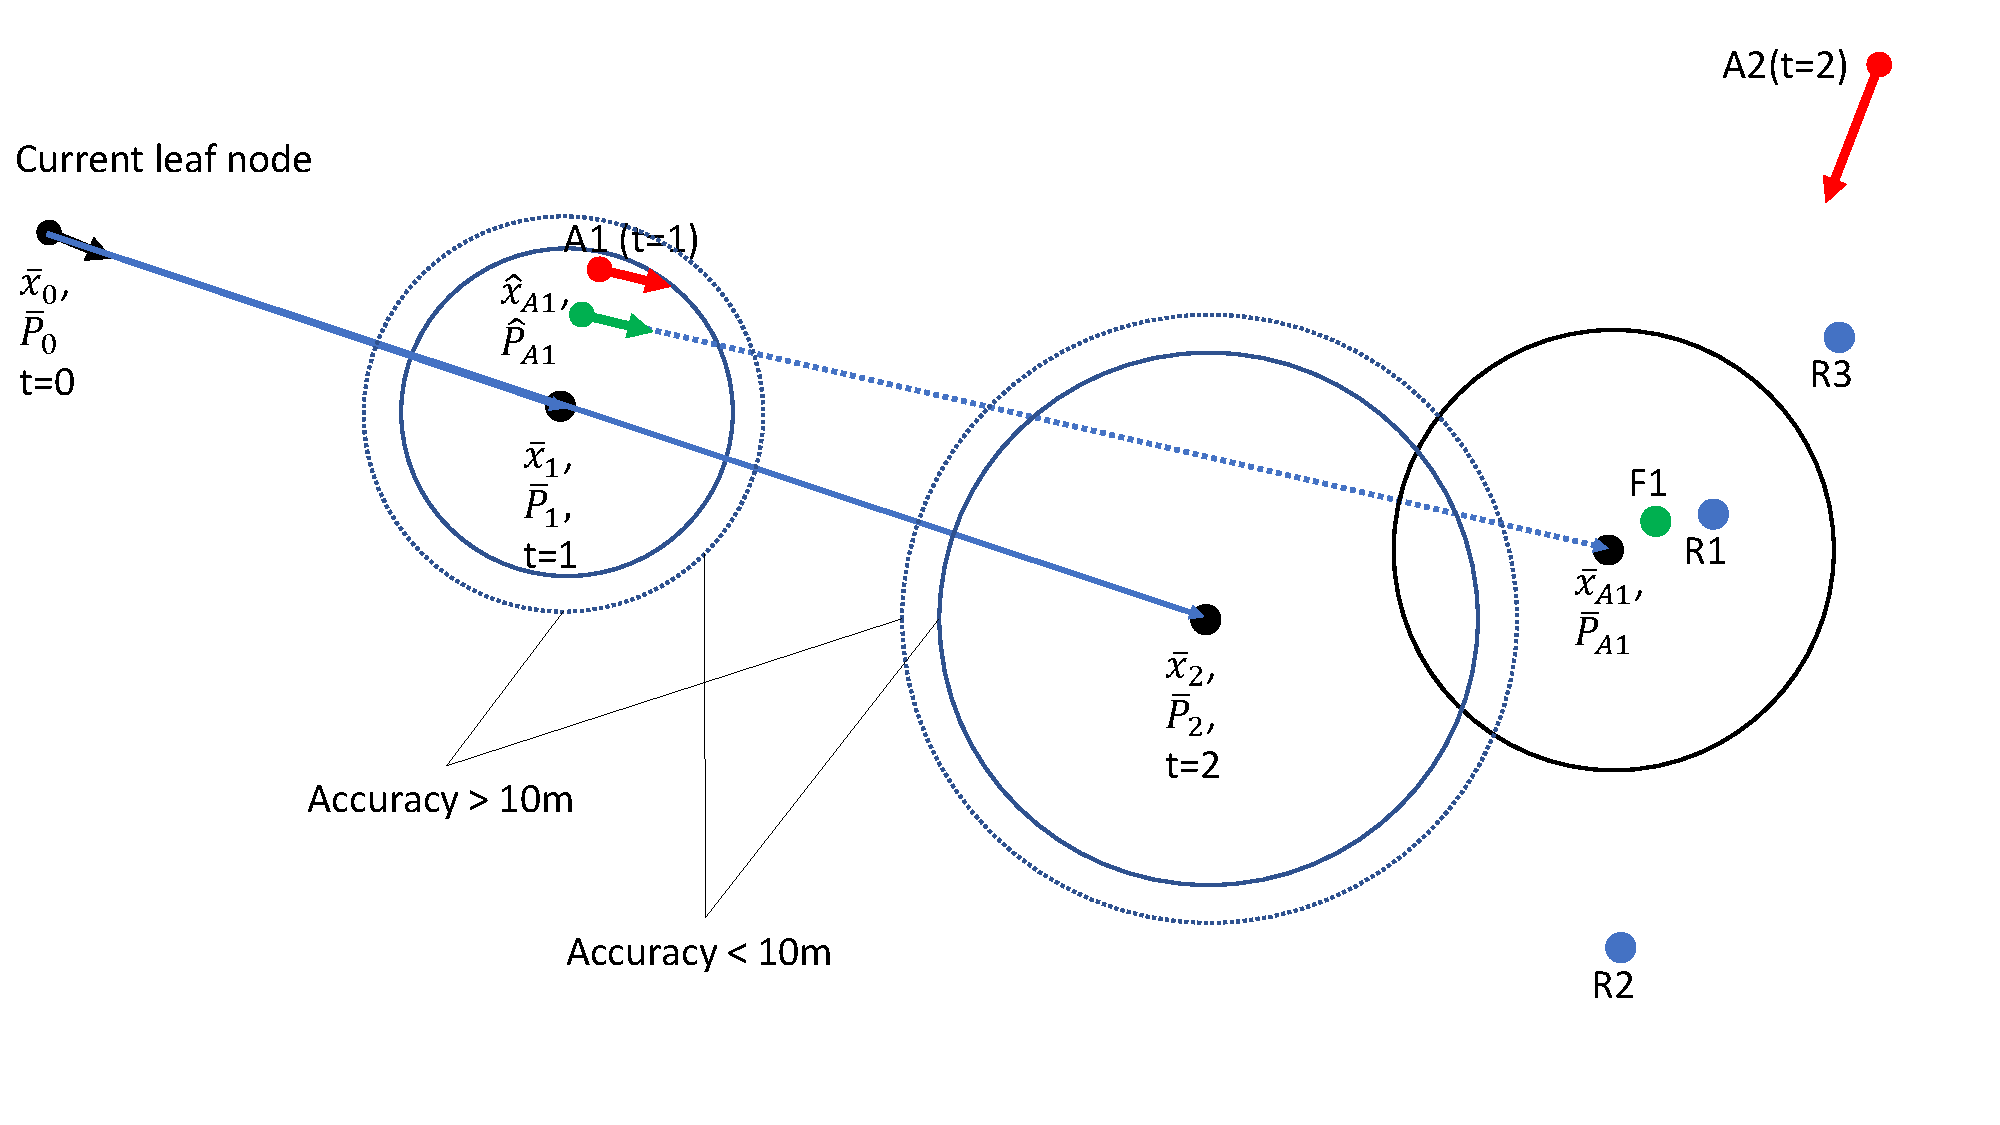
\includegraphics[width = .8\textwidth]{Figures/gating_at_ais_time.pdf}
\caption{Gating AIS at AIS time}\label{fig:gating_ais_at_ais_time}
\end{figure}
Figure~\ref{fig:gating_ais_at_ais_time} illustrates a situation where a single leaf node is showed in the upper left corner at \(t=0\), two red \gls{ais} measurements (A1 and A2) with position and velocity at \(t=1\) and \(t=2\) respectively and three blue radar measurements (R1, R2 and R3) at \(t=2.5\). \(\V{\bar{x}_1}\) and \(\V{\bar{x}_2}\) are the predicted states for \gls{ais} messages at \(t=1\) and \(t=2\) respectively, and the solid blue circles are representing the high accuracy gates while the dotted blue circles are representing the low accuracy gates. In this scenario only A1 is inside the \gls{ais} gates, and a filtered state \(\V{\hat{x}}_{A1}\) and covariance \(\M{\hat{P}}_{A1}\) is calculated. \(\V{\hat{x}}_{A1}\) is then predicted to \(t=2.5\) (\(\V{\bar{x}}_{A1}\) and \(\M{\bar{P}}_{A1}\)) and radar measurements are gated with the black solid circle based on the residual covariance to \(\M{\bar{P}}_{A1}\). Only R1 is inside this gate, thus a single fused hypothesis (F1) is created based on \(\V{\bar{x}}_{A1}\) filtered with R1.

\begin{figure}[H]
\centering
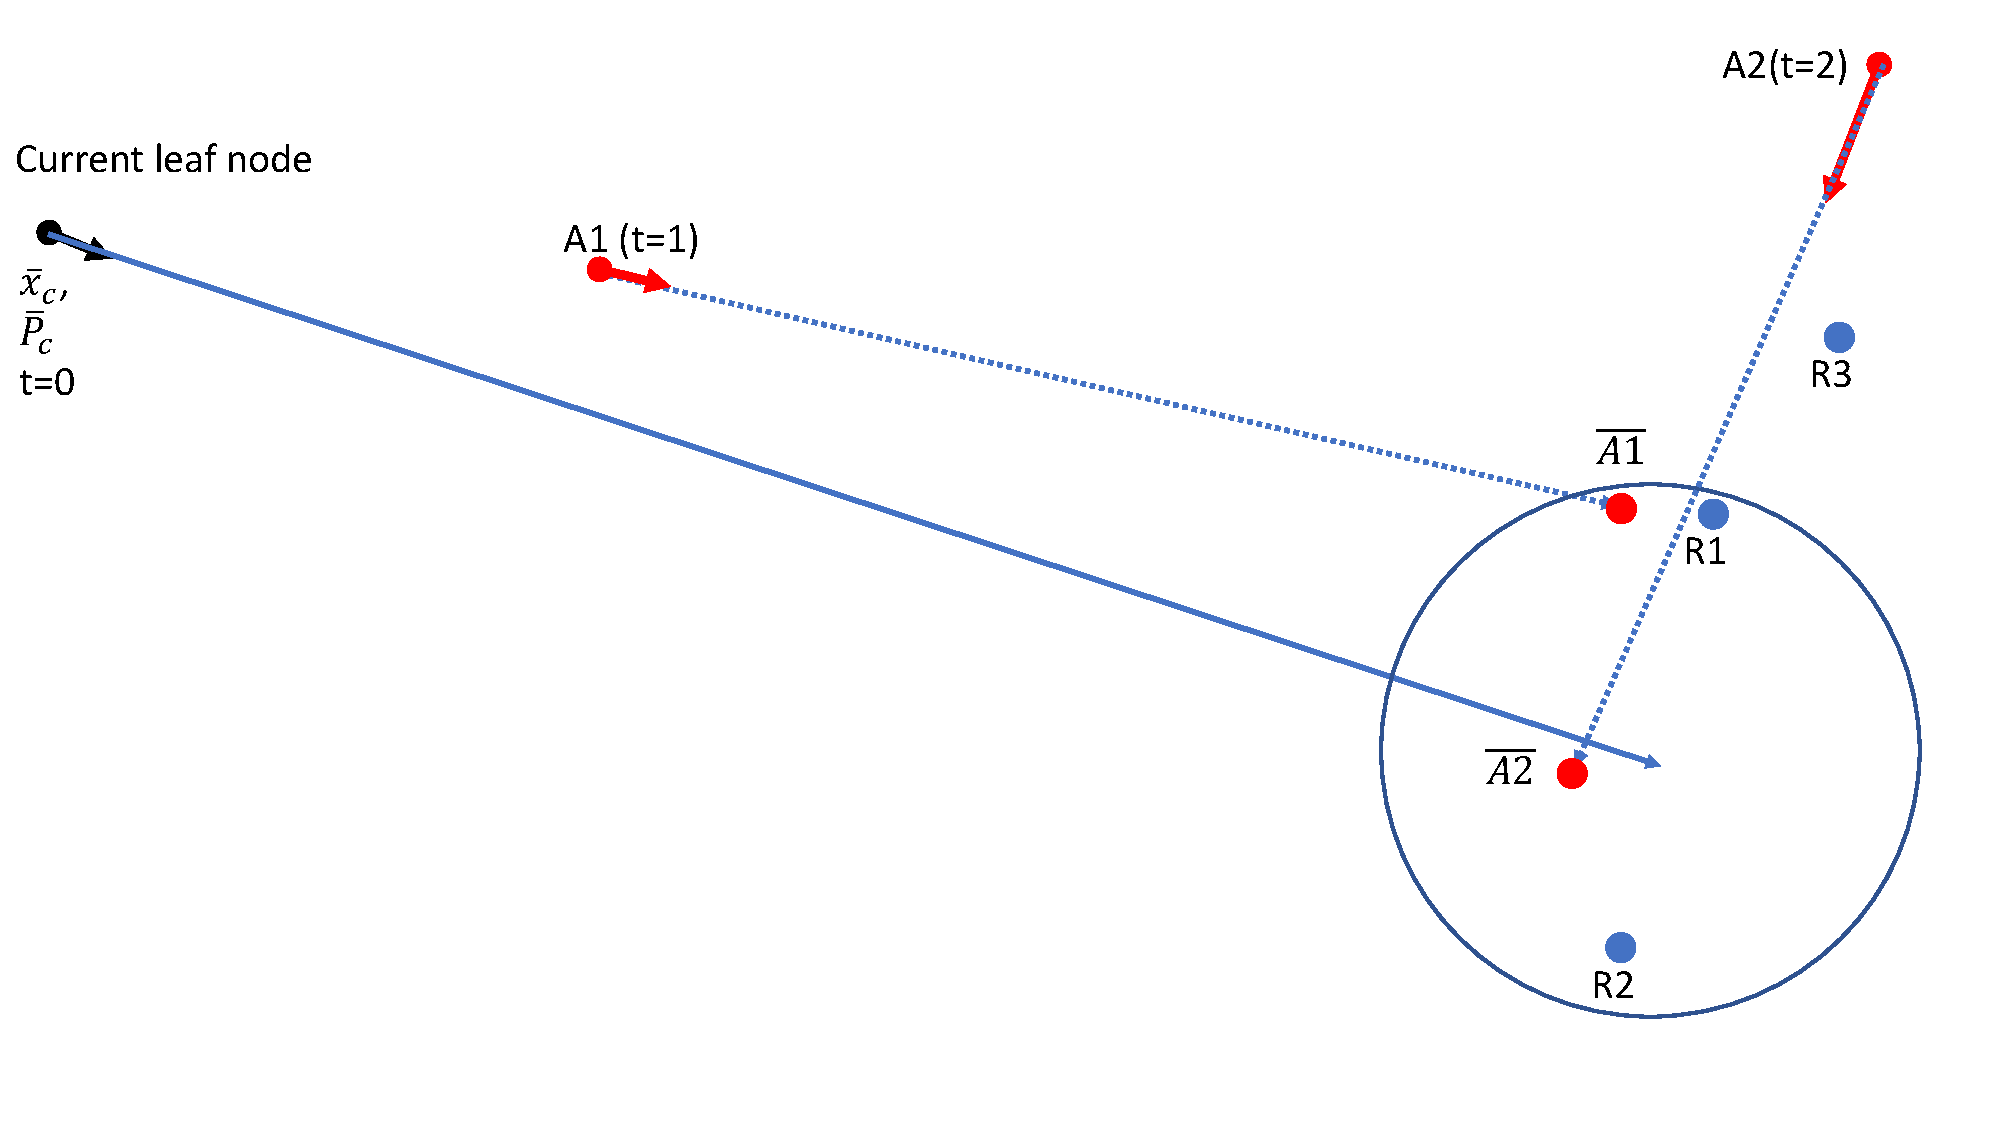
\includegraphics[width = .8\textwidth]{Figures/gating_at_radar_time.pdf}
\caption{Gating AIS at radar time}\label{fig:gating_ais_at_radar_time}
\end{figure}
If gating at radar time, all \gls{ais} measurements are predicted to radar time, and the predicted measurements are gated with the same gate at the radar measurements. By using the same gate on all measurements we assume that the radar measurement covariance is larger than the largest \gls{ais} measurement covariance, which is a reasonable assumption. This approach could however lead to unwanted AIS measurements inside the gate since the AIS measurements from other vessels can be predicted into the gate, thus leading to a more challenging association. This is exemplified in Figure~\ref{fig:gating_ais_at_radar_time}, where AIS measurement A2 would be inside the gate when gating at radar time but not if gating at \gls{ais} time. For all \gls{ais} measurements inside the gate, a complete set of fused hypotheses are created. In our example this would be (\(\overline{A1}\),R1), (\(\overline{A1}\), R2), (\(\overline{A2}\), R1) and (\(\overline{A2}\),R2). Since pure radar hypotheses are created prior to \gls{ais} processing it is not necessary to create any new pure radar hypotheses. 

In this work, the first approach is used for its assumed better performance and utilization of original data rather than predicted data. The \gls{ais} measurements are buffered between the radar scans, and pure \gls{ais} hypotheses are only created when no radar measurements fall inside the gate.

\subsection{Predict to AIS times}
To gate the AIS measurements, we first have to predict the target state and covariance (\ref{eq:predicted_origin_state_ais_time}) for each of the AIS time stamps (\ref{eq:ais_time_delta}) in the received AIS measurements. Since AIS only transmits a single integrity status, better or worse than 10 meter, maximum two possible \(\M{R}_{AIS}\) must be considered. With maximum two different time stamps and two different accuracies, a maximum of four different gates must be considered.
\begin{equation}\label{eq:ais_time_delta}
\begin{split}
\Delta T_{AIS_1} &= t_{AIS_1} - t_{c} \\
\Delta T_{AIS_2} &= t_{AIS_2} - t_{c} \\
\end{split}
\end{equation}

\begin{equation}\label{eq:predicted_origin_state_ais_time}
\begin{split}
\V{\bar{x}}_1 	&= \M{\Phi}(\Delta T_{AIS_1}) \V{x}_c \\
\M{\bar{P}}_1	&= \M{\Phi}(\Delta T_{AIS_1}) \M{P}_c \M{\Phi}^T(\Delta T_{AIS_1}) + \M{Q}(\Delta T_{AIS_1}) \\
\M{S}_{1_{High}}&= \M{H} \M{\bar{P}}_1 \M{H}^T + \M{R}_{AIS, High} \\
\M{S}_{1_{Low}}	&= \M{H} \M{\bar{P}}_1 \M{H}^T + \M{R}_{AIS, Low} \\
\V{\bar{x}}_2 	&= \M{\Phi}(\Delta T_{AIS_2}) \V{x}_c \\
\M{\bar{P}}_2	&= \M{\Phi}(\Delta T_{AIS_2}) \M{P}_c \M{\Phi}^T(\Delta T_{AIS_2}) + \M{Q}(\Delta T_{AIS_2}) \\
\M{S}_{2_{High}}&= \M{H} \M{\bar{P}}_2 \M{H}^T + \M{R}_{AIS, High} \\
\M{S}_{2_{Low}}	&= \M{H} \M{\bar{P}}_2 \M{H}^T + \M{R}_{AIS, Low} \\
\end{split}
\end{equation}

\subsection{Gate, filter and score}\label{sec:ais_gate_filter_score}
For each leaf node, all AIS measurements are gated with the gate matching their time, accuracy and threshold (Table~\ref{tab:chi_square_4_dof}). The measurements that pass the gating is then filtered with the predicted state and covariance matching its time, giving rise to an intermittent node (\ref{eq:filtered_ais_node}).
\begin{table}
\centering
\begin{tabular}{c c c c c c c c}
Confidence 	& 70\% 	& 80\% 	& 90\% 	& 95\% 	& 97.5\% 	& 99\% 	& 99.5\% \\ 
\midrule
\(\eta^2_{df=4}\) 	& 4.88 	& 5.99 	& 7.78 	& 9.49 	& 11.14 & 13.28	& 14.86
\end{tabular}\caption{Inverse \(\chi^2\) \gls{cdf} for four degrees of freedom}
~\label{tab:chi_square_4_dof}
\end{table}
\begin{equation}\label{eq:filtered_ais_node}
\V{\hat{x}}_1 = \V{\bar{x}}_1 + \M{K} \V{\tilde{z}}
\end{equation}

Depending on how we want the \gls{ais} to affect our tracking, two different scoring strategies are explored. The first approach is to view the \gls{ais} as a pure \emph{aiding}, where its only purpose is to improve the gating and uncertainty for the radar measurements. In this case, all \gls{ais} measurements are gated with a logarithmic score of zero, leading to neither improvement or worsening of the accumulative score of the track.

A second approach is to adapt the \gls{tomht} score function~\cite{Bar-Shalom2007} to the \gls{ais} paradigm. Since the \gls{ais} measurements are inherently labelled, then viewed from a single target, all \gls{ais} measurements except maximum one (depending on whether it have \gls{ais} transceiver or not) can be considered as clutter. If we then make the same assumptions as for radar measurements with respect to uniform spatial distribution and Poisson density distribution, we can estimate the expected number of \gls{ais} `clutter' measurements \( \lambda_{AIS} \) based on the amount of targets with \gls{ais} transmitters and the observation area (\ref{eq:ais_clutter_density}), where \(r_{radar}\) is the radar range. The clutter is in this context any measurement that does not belong to the target and which the target can erroneously utilize. The estimated clutter density could be calculated for a single frame, or averaged over a sliding window to reflect the \gls{ais} message flow over time since \gls{ais} transmission is not synchronised with the radar period. The resulting score function becomes (\ref{eq:ais_score_function2}).

\begin{equation}\label{eq:ais_clutter_density}
\lambda_{AIS} = \frac{n_{AIS}}{\pi r_{radar}^2}
\end{equation}

\begin{equation}\label{eq:ais_score_function2}
\mathrm{NLLR}_{AIS} = \frac{1}{2} NIS + \ln \lambda_{AIS} |2 \pi S|^{1/2} 
\end{equation}

Testing has shown that both the first and last method gives an improvement over pure radar tracking, and since the last method gives a little more improvement since it scores the \gls{ais} measurements with a reasonable values compared to the radar measurements, hence not giving the \gls{ais} measurements an enormous advantage or disadvantage. The second method is used in all the simulations in Chapter~\ref{chapter:results}.

\subsection{Predict to radar time}
All gated and filtered states from Section~\ref{sec:ais_gate_filter_score} is then predicted forward to the time of the radar measurements. This time delta will differ based on the time of the AIS measurement. Radar measurements are then gated for each predicted state and covariance, whereon a fused hypothesis are created for each radar measurement inside the gate. If there is no radar measurements inside the \gls{gate}, a pure \gls{ais} hypothesis are created. 

\subsubsection{Fused hypotheses}
The predicted state and covariance is then filtered with the gated radar measurement according to (\ref{eq:kalman_measurement_update}). The radar measurement is scored according to (\ref{eq:radar_score_function}), and the hypothesis score is a weighted sum of the AIS and radar score (\ref{eq:weighted_score}).
\begin{equation}\label{eq:weighted_score}
\mathrm{NLLR} = \frac{1}{2} \mathrm{NLLR}_{AIS} + \frac{1}{2} \mathrm{NLLR}_{Radar}
\end{equation}

\subsubsection{Pure AIS hypotheses}\label{subsec:pure_ais_hypotheses}
If no radar measurements are present in the gate, pure AIS hypotheses are created. This can be the situation when a target is broadcasting an AIS message, but is either in radar shadow or is not detected by the radar for any reason. These hypotheses are not created when one or more radar measurements are available, based on the assumption that if a radar measurement is present, the difference between a fused hypothesis and a pure AIS hypothesis is quite small since the AIS measurement covariance typically will be much smaller than the radar measurement covariance, leading to a fused state very close to the AIS measurement. The pure AIS hypothesis will use its predicted state and covariance and be  scored with \(\mathrm{NLLR}_{AIS}\), somewhat similar to radar zero hypotheses.

\section{Clustering}
The problem of finding the globally optimal set of track hypotheses increases exponentially with the number of hypotheses in the problem. To reduce the size of the problem, it is desirable to split it into smaller independent problems. Both because it enables parallel computation and it reduces the total cost of solving the problem. Track trees that have common measurements must be solved together, since they can have mutual exclusive leaf nodes. The clustering can be done efficiently through \gls{bfs} or \gls{dfs} on a graph made from the \gls{track hypothesis tree}.

By constructing a 0--1 adjacency matrix describing the connection between all the nodes in the \gls{track forest}, the clustering problem is equivalent to the \emph{connected components} problem in graph theory~\cite{Chen2015}.

\section{Optimal data association}\label{sec:optim_data_association}
The aim of this section is to elaborate the use of ILP to solve the data association problem in MHT that arises when there are multiple, possibly mutually exclusive, possibilities of measurement arrangements within the existing set of tracks. When the targets are divided into independent clusters, each of them can be treated as a global problem where we want to minimize the cost or maximize the score of the selected \glspl{track hypothesis} (leaf nodes). The selected \glspl{track hypothesis} must also fulfil the constraints, that each measurement can only be a part of one track, and that exactly one track hypothesis must be selected from each target. Since only binary values, selected or not selected, is possible for selection of hypotheses, the problem becomes an \gls{ilp}. In the case where a cluster is only containing one target tree, the best hypothesis can be selected by running a search among the leaf nodes after the highest score, since none of the leaf nodes are excluding other leaf nodes in other target trees. This will often be the case for targets that are largely spaced out, and their gates are not and have not overlapped in a while. For any other case, where there are two or more targets in a cluster, the procedure in Section~\ref{subsec:integer_linear_programming} must be carried out.

\subsection{Integer Linear Programming}\label{subsec:integer_linear_programming}
The essence of any optimization problem is a cost function and a set of constraints. In our problem, we want to select the combination of hypotheses (leaf nodes) that gives the highest score / lowest cost, while not selecting any measurement more than one time and ensure that we select minimum and maximum one hypothesis from each target. 

Our score function is the sum of the selected node scores, and since we are using negative logarithmic scores the goal is to minimize the overall score, making the problem a minimum cost problem. Our cost vector \(\V{c}\) is made up from the scores of all the leaf nodes in the forest build by the trees clustered together, arranged in the order they are visited by a \gls{dfs}. The accompanying selection vector \( \V{\tau} \) is of the same dimension with boolean values, where the selected hypotheses are value 1 and all other is value 0. These two together form the objective function (\ref{eq:objective_funtion}).
\begin{equation}
\begin{aligned}
& \underset{\V{\tau}}{\text{min}}
& & \V{c}^T \V{\tau}
\end{aligned}
\label{eq:objective_funtion}
\end{equation}

To ensure that we are selecting the same measurement maximum one time, a binary matrix \( \M{A_1} \) describing the association between nodes and measurements are created.\(\M{A_1}\) has as many rows are there are unique real measurement in the cluster forest and as as many columns as there are track hypotheses. All radar- and AIS measurement are real measurement, whereas dummy nodes do not contain any real measurements. Each rows in \( \M{A_1} \) represents a real measurements that exists in the cluster forest, and each column represents a track hypothesis. For each track hypothesis are the rows that represents the measurements used by that track hypothesis given value 1 (True) to indicate the usage. All other rows for that column are given value 0 (False) to indicate that it does not use these measurements. The order of the columns in \( \M{A_1} \) is the same as the rows in \( \V{c} \) and \( \V{\tau} \). Since we are only limiting a maximum of one usage of each measurement and no minimum, the constraint becomes an inequality constraint (\ref{eq:inequality_constraint}) where \( \V{1} \) is a vector of ones with the same dimension as \( \V{\tau} \).
\begin{equation}\label{eq:inequality_constraint}
\M{A_1} \V{\tau} \leq \V{1}
\end{equation}

The second constraint we need to impose is that we need to select exactly one track hypothesis from each tree. This can be done by creating a boolean matrix \( \M{A_2} \) which describes the relationship between hypotheses and trees / targets. \( \M{A_2} \) will have as many rows as there are targets in the cluster, and columns as \( \M{A_1} \). The intersections between hypotheses and targets that belong together is value 1, all other is value 0. Since this constraint has a fixed requirement, it is formulated as an equality constraint (\ref{eq:equality_constraint}) with \( \V{1} \) as in (\ref{eq:inequality_constraint}).
\begin{equation}\label{eq:equality_constraint}
\M{A_2} \V{\tau} = \V{1}
\end{equation}

The complete \gls{ilp} formulation becomes (\ref{eq:optim_formulation}), where \(\V{\tau}\) is a binary vector with dimension equal the number of leaf nodes in the track forest.
\begin{equation}
\begin{aligned}
&	\underset{\V{\tau}}{\text{max}}
&&	\V{c}^T \V{\tau} \\
&	\text{s.t.}
&&	\M{A_1} \V{\tau} \leq \V{b_1} 	\\
&&&	\M{A_2} \V{\tau} = \V{b_2}	\\
&&&	\V{\tau} \in {\{0,1\}}^{M}
\end{aligned}
\label{eq:optim_formulation}
\end{equation}

An example based on Figure~\ref{fig:hyp_forest} at time step 2, where the \(\M{A}\) matrices and \(\V{C}\) vector would be (\ref{eq:example_matrices}).
\begin{figure}[H]
\centering
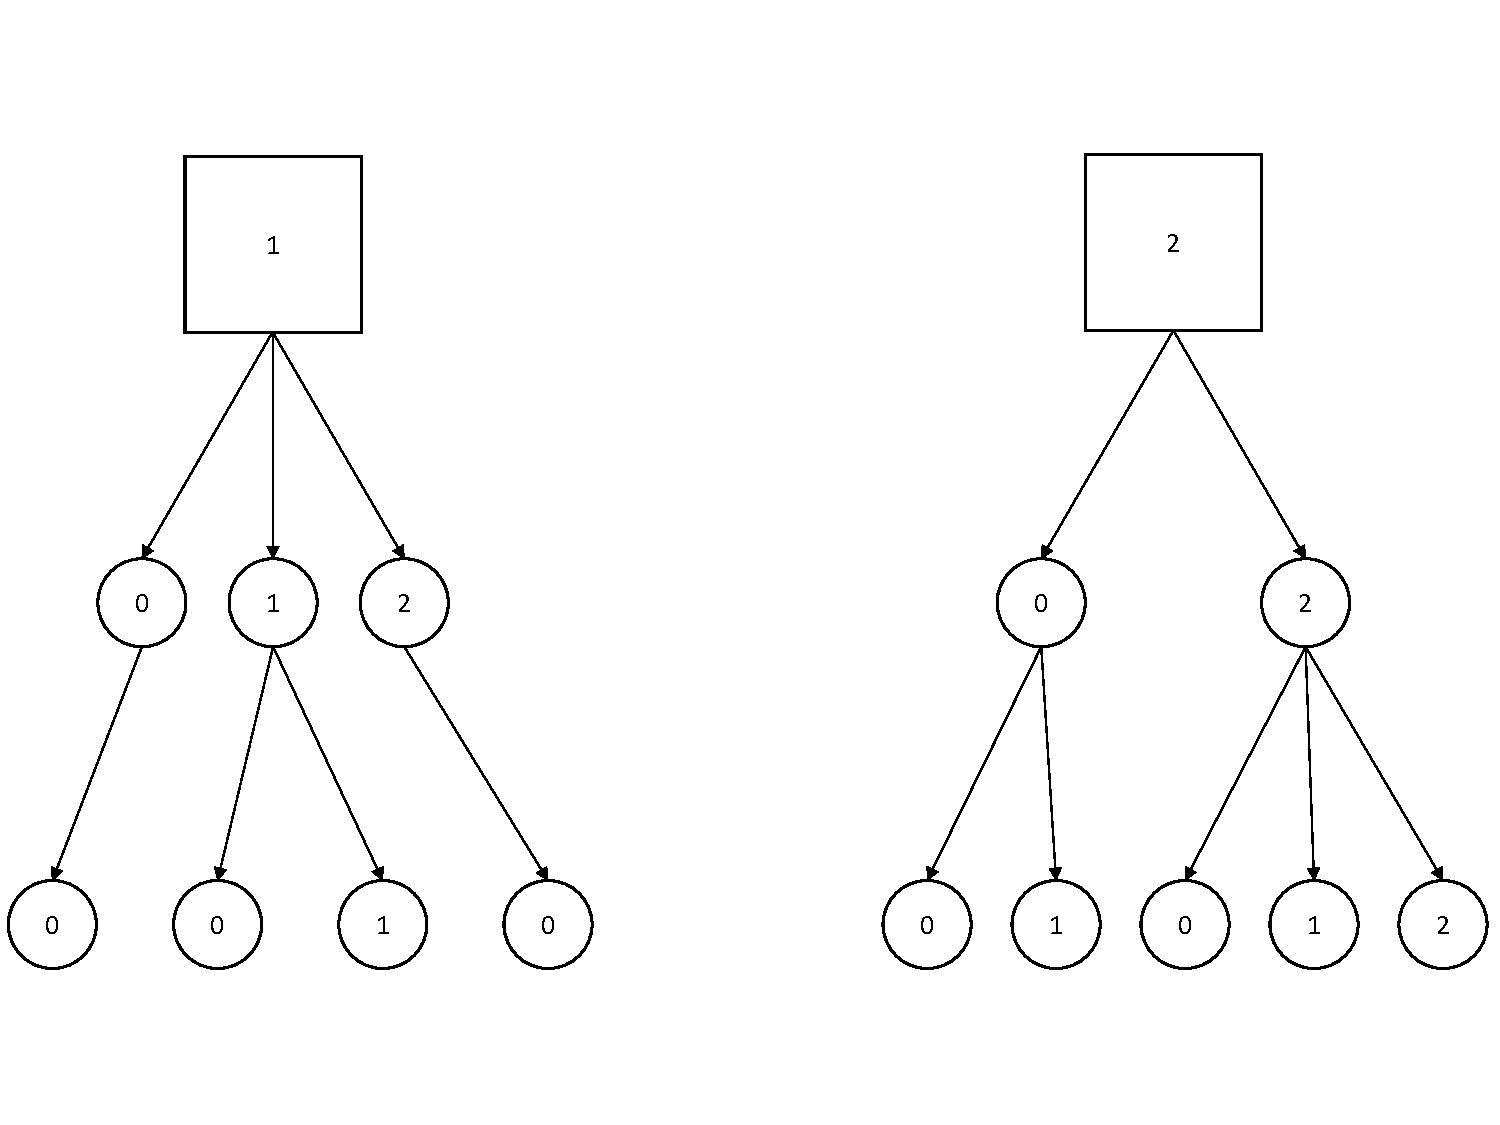
\includegraphics[clip, trim=0cm 2.5cm 0cm 2.5cm, width = .7\textwidth]{Track-forest}
\caption{Track hypotheses forest}\label{fig:hyp_forest}
\end{figure}

\begin{equation}
\begin{split}
\M{A_1} &=\begin{bmatrix}
		0 & 1 & 1 & 0 & 0 & 0 & 0 & 0 & 0 \\
       	0 & 0 & 1 & 0 & 0 & 1 & 0 & 1 & 0 \\
       	0 & 0 & 0 & 1 & 0 & 0 & 1 & 1 & 1 \\
       	0 & 0 & 0 & 0 & 0 & 0 & 0 & 0 & 1 \\
     	\end{bmatrix},\quad
\V{b_1} = 	\begin{bmatrix}
			1 \\ 1  \\ 1 \\ 1
			\end{bmatrix} \\
\M{A_2} &=\begin{bmatrix}
		1 & 1 & 1 & 1 & 0 & 0 & 0 & 0 & 0 \\
       	0 & 0 & 0 & 0 & 1 & 1 & 1 & 1 & 1 \\
     	\end{bmatrix} ,\quad
\V{b_2} = 	\begin{bmatrix}
			1 \\ 1
			\end{bmatrix} \\
\V{c} &=\begin{bmatrix}
		\lambda_1 & \lambda_2 & \lambda_3 & \lambda_4 & \lambda_5 & \lambda_6 & \lambda_7 & \lambda_8 & \lambda_9
		\end{bmatrix}^T \\
\end{split}
\label{eq:example_matrices}
\end{equation}

\subsection{Solvers}
The problem (\ref{eq:optim_formulation}) is formulated on standard form, which enables the use of existing off-the-shelf ILP solvers. There are a lot of off-the-shelf \gls{ilp} and \gls{milp} solvers on the marked, both free open source and commercial. The performance difference of some solvers were tested in~\cite{Liland_2017}, where the difference where found marginal,  most likely because each optimization problem is relatively small and the initialization and preprocessing of the solver and problem played a significant part of the runtime compared to the actual solving. In this work, Google Optimization Tools is used as interface between the programming language and the solver. The default solver CBC was used exclusively in this work as its performance was on par with the others tested in~\cite{Liland_2017}. 

\section{N-Scan pruning}
To keep the computational cost within reasonable limits, it is necessary to limit the amount of time steps backwards in time that the algorithm computes. This is done by removing all branches but the active track hypothesis at the current root node, and assign the one remaining node as new root node. This procedure is graphically explained in Figure~\ref{fig:pruned_tree}, where a solid square frame indicates the current root node, and a dotted square frame indicates the new root node. The bold arrows in the figure represents the active track.
\begin{figure}
\centering
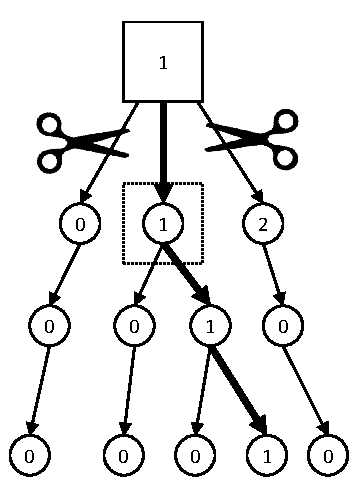
\includegraphics[scale = .8]{Figures/Pruned-tree.pdf}
\caption{N-scan pruning}\label{fig:pruned_tree}
\end{figure}

\subsection{Dynamic window}
For any MHT to be realistic over time it need to have a sliding window removing the unused hypotheses N steps back in time. The sliding window size (N) could be a static design parameter or a function of the runtime of that tree, which reflects the overall size of the tree. This enables the system to adapt its core parameters to guarantee its runtime demands. This scaling of N proved itself very efficient through testing and development, but is disabled in Chapter~\ref{chapter:results} for true comparison between different windows sizes.

\section{Track termination}
Since targets can disappear from the observation region both by leaving the radar range and by driving behind objects that puts them in a radar shadow, it is necessary to terminate these tracks. It is also desirable to terminate falsely initiated tracks as soon as possible, since a guidance system would steer clear of any objects reported to it. The first scenario, where the target is leaving the radar range can easily be detected and the track can be terminated quickly based on the predicted position of the target relative to our own position. The second scenario, can be approached in different ways depending on the available data and computational power. The simplest solution is to terminate all tracks where the selected node after each iteration have a score higher that a threshold. This could terminate tracks with consecutive miss detections, which is desirable for false tracks, but can lead to premature termination of true targets with temporarily low \gls{Pd}. This means that the termination threshold becomes a trade-of between killing false tracks and keeping targets with lower \gls{Pd} and shadowed targets. 

A more advanced approach could be to utilize map data to estimate whether or not a target is in a radar shadow of land objects, and then make a decision on whether this target should be given a lower \gls{Pd} temporary or terminated based. This could also be done between targets if target extent is estimated, where targets behind other targets are given a lower \gls{Pd} to punish miss detections less.

In this work, only range and score termination is implemented.

\section{Track smoothing}
After each iteration of the MHT algorithm a track list based on the selected hypotheses from Section~\ref{sec:optim_data_association} is passed forward to the operator and guidance system. Both human operators and guidance systems will try to predict the targets' behaviour based on their historical track. To improve the visualisation for this purpose it is possible to smooth the tracks based on the real measurements in the track and masking the dummy measurements in a Kalman smoother~\cite{Brown2012} with the same model as used in the predictions. As illustrated in Figure~\ref{fig:track_smoothing}, this will lead to a smother and in most cases a more accurate representation of the true track since it avoids the straight lines caused by dead reckoning. The circles represent dummy measurements, while it is real measurements on both sides of the dead reconing period (not plotted to avoid cluttered illustration). Figure~\ref{fig:track_smoothing_zoomed} is the same image zoomed in around the dead reconing area. This smoothing will however not affect the \gls{tracking} performance since it is done after miss detections are corrected and only on the track list sent out of the tracking module.
\begin{figure}[H]
\centering
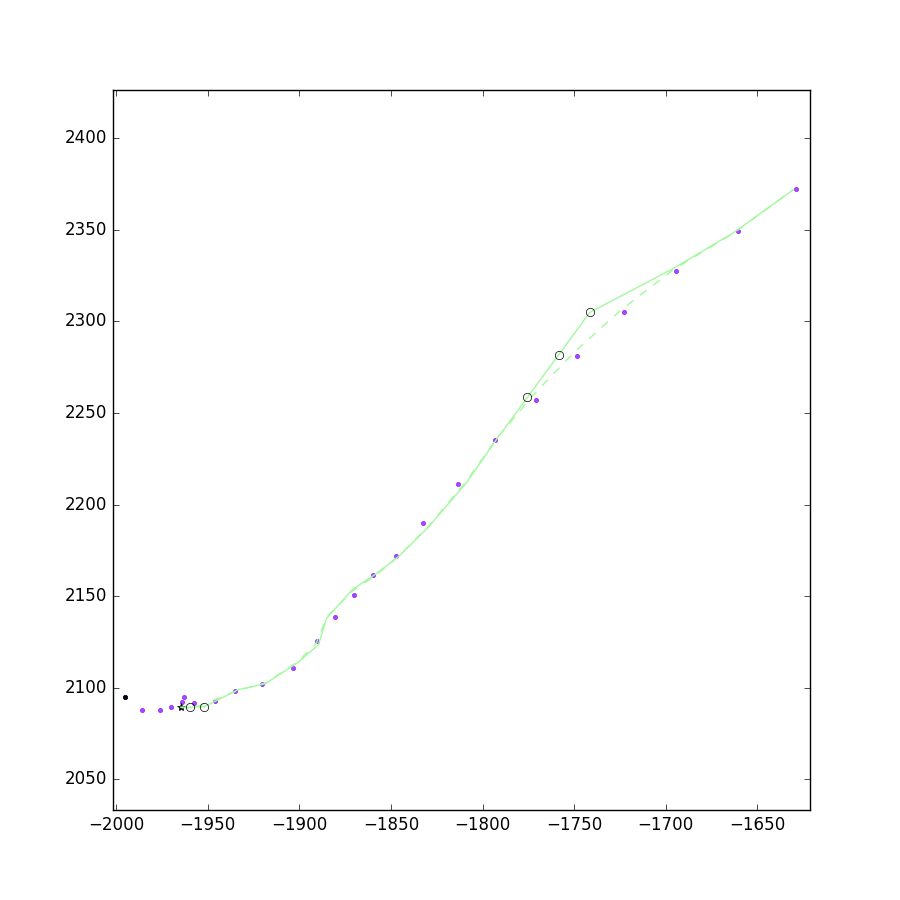
\includegraphics[trim={10cm 11cm 4cm 4cm},clip=true,height = .4\textheight]{Figures/track_smoothing_dummy_markers.png}
\caption{Track smoothing zoomed}\label{fig:track_smoothing_zoomed}
\end{figure}

\begin{figure}
\centering
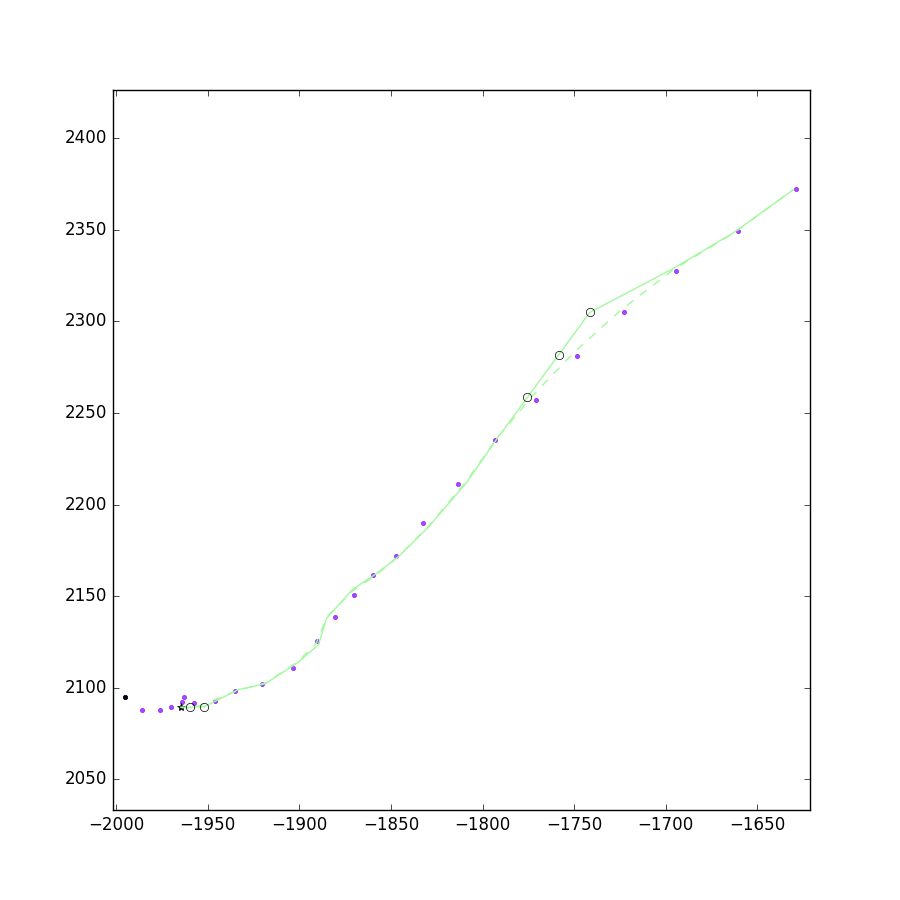
\includegraphics[width = .9\textwidth]{Figures/track_smoothing_dummy_markers.png}
\caption{Track smoothing}\label{fig:track_smoothing}
\end{figure}
